\chapter{INTRODUCTION}
In this study, an online RC Car Battle framework is proposed. The project aims in designing two robot cars that can be operated using Android mobile phones and playing online shooter game with these two remote controlled cars. The controlling of the robot car is done wireless through Android smart phone using the Bluetooth feature present in it. This paper presents the hardware and software design decisions and methods applied on the system. \\

\section{Project Definition}

In this project, two remote controlled cars, remote control Android application have been developed. The remote control application connects to the target phone via Bluetooth communication for driving the robot car, and provides online game between two robot cars by connection via real time database. Robot cars have IR transmitter and IR receiver, that are used for shooting procedure in the game. There is a IR transmitter in the front of the robot car and there is a IR receiver in the back of the car. If IR receiver detects a IR light on it, that means the related car has been hit. So If a user wants to shoot the target car, the user should go to the back of the opponents car, and trigger the IR transmitter in order to hit the opponent. These procedure is shown in the Figure \ref{fig:frog}. All of these controls (connecting, driving, triggering the IR transmitter) has done by remote control Android application.

\begin{figure}[!htbp]
    \centering
    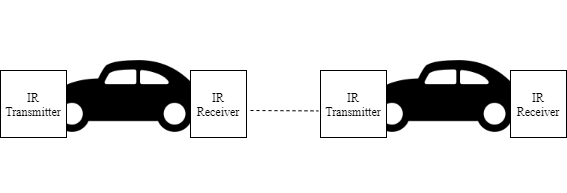
\includegraphics[width=0.9\textwidth]{Imgs/ir_diagram.png}
    \caption{\label{fig:frog}IR Receiver and Transmitter on RC Battle}
\end{figure}

\section{Project Requirements}
The requirements within the scope of the project are mentioned in this section. Project requirements are grouped under two separate headings as system requirements and functional requirements.

\subsection{Functional Requirements}
\begin{enumerate}
    \item Users should be able to connect to the RC car using remote control application which was developed within the scope of this project via Bluetooth.
    \item Users should be able to control the steering of the RC car using gyroscope and accelerometer of the phone.
    \item Users should be able to view the current steering angle on the user interface of the application.
    \item Users should be able to control the speed of the car by using slider on the user interface in both directions (forward and backward).
    \item Users should be able to view the current Li-Po battery charge percentage on the user interface of the application.
    \item Users should be able to trigger the IR transmitter of the RC car on the user interface of the application.
    \item After communication loss or non-healthy communication with the target RC Car, the RC car must stop all motors for safety with predefined threshold time.
    \item Users should be able to connect the online game server (database) on the user interface of the application.
    \item Users should be able to see the current score on the user interface of the application.
    \item A RC car should be able to hit the opponent RC car at least 1.5 meter away with IR transmitter of it.
\end{enumerate}

\subsection{System Requirements}
This section contains the system requirements of project, which are hardware requirements of the RC car robot and the remote controller application. Hardware and related electronic components discussed detailed in the section \ref{sec_hardware_design}\\

\begin{enumerate}
    \item STM32 Nucleo-64 development board.
    \item L298N Motor Driver, STMicroelectronics\texttrademark.
    \item HC05 Bluetooth\texttrademark\;module
    \item 5V 3A voltage regulator.
    \item 3S Li-Po Battery. Minimum capacity is 850 mAh.
    \item Bidirectional DC motor for accelerating.
    \item MG90s 50 Hz servo motor for steering. 
    \item IR receiver and IR transmitter module.
    \item Android\texttrademark\;smartphone with at least version Android 5.0.
\end{enumerate}
